% Copyright 2007 by Till Tantau
%
% This file may be distributed and/or modified
%
% 1. under the LaTeX Project Public License and/or
% 2. under the GNU Public License.
%
% See the file doc/licenses/LICENSE for more details.



\documentclass{beamer}

% Setup appearance:

\usetheme{}


% Standard packages

\usepackage[english]{babel}
\usepackage{amsmath}
\usepackage{amssymb}
\usepackage{graphicx}
\usepackage{subfigure}
\usepackage{color}
\usepackage{amsbsy}
\usepackage{verbatim}
\setbeamertemplate{footline}[frame number]

% Author, Title, etc.

\title{An introduction to Bayesian modeling \\
using R and JAGS}

\author{
  Instructors \\
  Kent~Holsinger \\
  Xiaojing~Wang % \inst{1}
  \vskip 2mm % \inst{1} \\
  \textit{University of Connecticut}
  \vskip 2mm
  ~~\textit{}
 }

 \date{22 July 2015}




% The main document

\begin{document}

\begin{frame}
  \titlepage
\end{frame}

\begin{frame}{Overview of the Workshop}

\begin{itemize}

\item Focus on using R and JAGS for Bayesian analysis

\item Linear regression including mixed modeling -- Kent Holsinger

\begin{itemize}

\item Simple linear regression

\item Multiple regression (including random effects)

\end{itemize}

\item Multicollinearity -- Xiaojing Wang

\begin{itemize}

\item Hierarchical independent prior distributions

\item Variable selection

\end{itemize}

\end{itemize}

\end{frame}

\begin{frame}{Linear Regression}

One of the most common statistical procedures in ecology and
evolution. For example,

\begin{itemize}
\item Data on LMA from 535 individuals in the genus {\it Protea\/}~(42
  species, 48 sites, 142 unique site/species combinations)
\item Data on mean annual temperature for each of those sites
\end{itemize}

\begin{center}
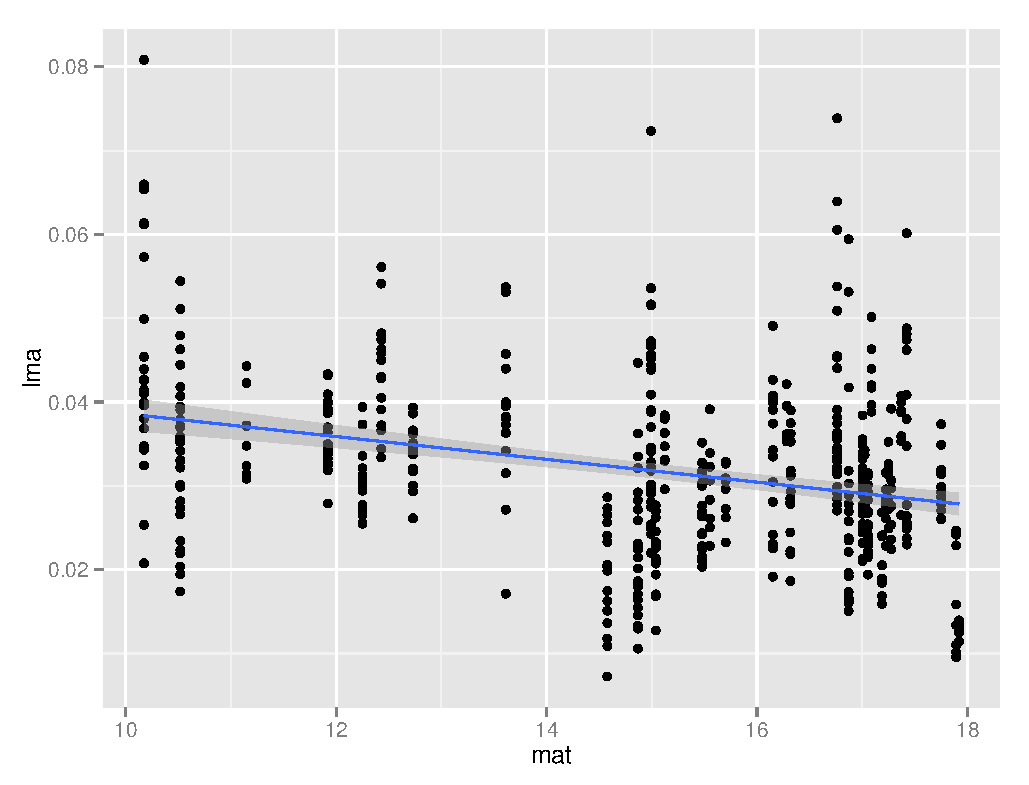
\includegraphics[height=5.5cm]{lma-vs-mat.pdf}
\end{center}

\end{frame}

\begin{frame}[fragile]{Linear Regression}
In R
{\tiny
\begin{verbatim}
> summary(lm(lma ~ mat, data=tmp))

Call:
lm(formula = lma ~ mat, data = tmp)

Residuals:
      Min        1Q    Median        3Q       Max
-0.025126 -0.005781 -0.000785  0.004647  0.044444

Coefficients:
              Estimate Std. Error t value Pr(>|t|)
(Intercept)  0.0521895  0.0027116  19.246  < 2e-16 ***
mat         -0.0013587  0.0001785  -7.611 1.24e-13 ***
---
Signif. codes:  0 �***� 0.001 �**� 0.01 �*� 0.05 �.� 0.1 � � 1

Residual standard error: 0.009815 on 533 degrees of freedom
Multiple R-squared:  0.09803,	Adjusted R-squared:  0.09634
F-statistic: 57.93 on 1 and 533 DF,  p-value: 1.241e-13
\end{verbatim}
}

\end{frame}

\begin{frame}{Linear Regression}

Remember basic assumptions of simple linear regression

\begin{eqnarray*}
y_i &=& \beta_0 + \beta_1x_i + \epsilon_i \\
\epsilon_i &\sim& \mbox{N}(0, \sigma^2)
\end{eqnarray*}

Here's another way to write that

\begin{eqnarray*}
y_i &\sim& \mbox{N}(\mu_i, \sigma^2) \\
\mu_i &=& \beta_0 + \beta_1x_i
\end{eqnarray*}

The second way of writing the model will be more convenient for us, so
that's the approach we'll use.

\end{frame}

\begin{frame}{Statistical Analysis}
  Statistical inference is the process of learning about the general
  characteristics of a population from a sample.
\begin{itemize}
\item Characteristics often expressed in terms of parameters $\theta$.
\item Measurements on the subset of members given by numerical values $Y$.
\item Before the data are observed, both $Y$ and $\theta$ are unknown.
\item A probability model is assumed for observed data if we knew $\theta$ is the truth.
\item What if we have prior information about $\theta$?
\end{itemize}
\end{frame}

\begin{frame}{Bayesian Inference}
  Bayesian inference allows us to update prior beliefs with the
  observed data to quantify uncertainty about $\theta$.
\begin{itemize}
\item Prior Distribution: $p(\theta)$
\item Sampling Model (likelihood): $p( y \mid \theta)$
\item Posterior Distribution
\[
	p(\theta \mid y)=\frac{p(y \mid \theta) p (\theta)}{p(y)}
\]
\item Calculating $p(y)$ is typically very challenging. Use MCMC
  (implemented in JAGS) to estimate $p(\theta \mid y)$.

\end{itemize}
\end{frame}

\begin{frame}{Metropolis-Hastings Algorithm}
For $\theta_j$
\begin{itemize}
\item Propose a new $\theta_j^*\sim q(\theta_j^{(t)} | \theta_j^t)$
\item Calculate Metropolis-Hastings ratio
\[
\alpha=\frac{p({Y}|\theta_j^*)p(\theta_j^*)/q(\theta_j^*|\theta_j^{(t)})}{p({Y}|\theta_j^{(t)})p(\theta_j^{(t)})/q(\theta_j^{(t)}|\theta_j^*)}
\]
\item if $\alpha<1$ set
\[
\theta_j^{(t+1)}=\left\{
\begin{array}{ll}
\theta_j^*& \mbox{with probability $\alpha$}\\
\theta_j^{(t)} & \mbox{with probability $1-\alpha$}
\end{array}
\right.
\]
If $\alpha>1$ set $\theta_j^{(t+1)}=\theta_j^{*}$
\item Repeat for $j=1,\dots,J$
\item Repeat for $t=1,\dots,T$
\end{itemize}

\end{frame}

\begin{frame}{Linear Regression - as a Bayesian}

We start with the sampling model $p(y \mid \theta)$, where $\theta=(\beta_0, \beta_1, \sigma^2)'$, 
\begin{eqnarray*}
y_i &\sim& \mbox{N}(\mu_i, \sigma^2) \ , \\
\mu_i &=& \beta_0 + \beta_1x_i \ , 
\end{eqnarray*}
and $x_i$ is the value of the covariate in individual $i$. Then we
add prior distributions $p(\theta)$, 
\begin{eqnarray*}
\beta_0 &\sim& \mbox{N}(0, \tau^{-1}), \\
\beta_1 &\sim& \mbox{N}(0, \tau^{-1}), \\
\sigma^2 &=& \frac{1}{\tau_{resid}}, \\
\tau_{resid} &\sim& \mbox{Gamma}(1,\phi)
\end{eqnarray*}
\end{frame}

\begin{frame}[fragile]{Linear Regression - in R+JAGS\footnote{simple-linear-regression.jags}}

\begin{itemize}

\item Rescale all variables to mean of 0, standard deviation of 1

{\tiny
\begin{verbatim}
Inference for Bugs model at "simple-linear-regression.jags", fit using jags,
 5 chains, each with 10000 iterations (first 5000 discarded), n.thin = 5
 n.sims = 5000 iterations saved
             mu.vect sd.vect     2.5%      25%      50%      75%    97.5%  Rhat n.eff
beta.0         0.000   0.041   -0.082   -0.028    0.000    0.028    0.080 1.001  5000
beta.mat      -0.313   0.041   -0.393   -0.341   -0.314   -0.285   -0.231 1.002  1900
sigma.resid    0.953   0.029    0.897    0.933    0.952    0.972    1.012 1.001  3700
\end{verbatim}
}
\item Compare with lm() results from R
{\tiny
\begin{verbatim}
              Estimate Std. Error t value Pr(>|t|)
(Intercept)  8.614e-17  4.110e-02   0.000        1
mat         -3.131e-01  4.114e-02  -7.611 1.24e-13 ***

Residual standard error: 0.9506 on 533 degrees of freedom
\end{verbatim}
}
\end{itemize}

\end{frame}

\begin{frame}{Robust Regression}

\begin{itemize}

\item What do we do with outliers?

\begin{center}
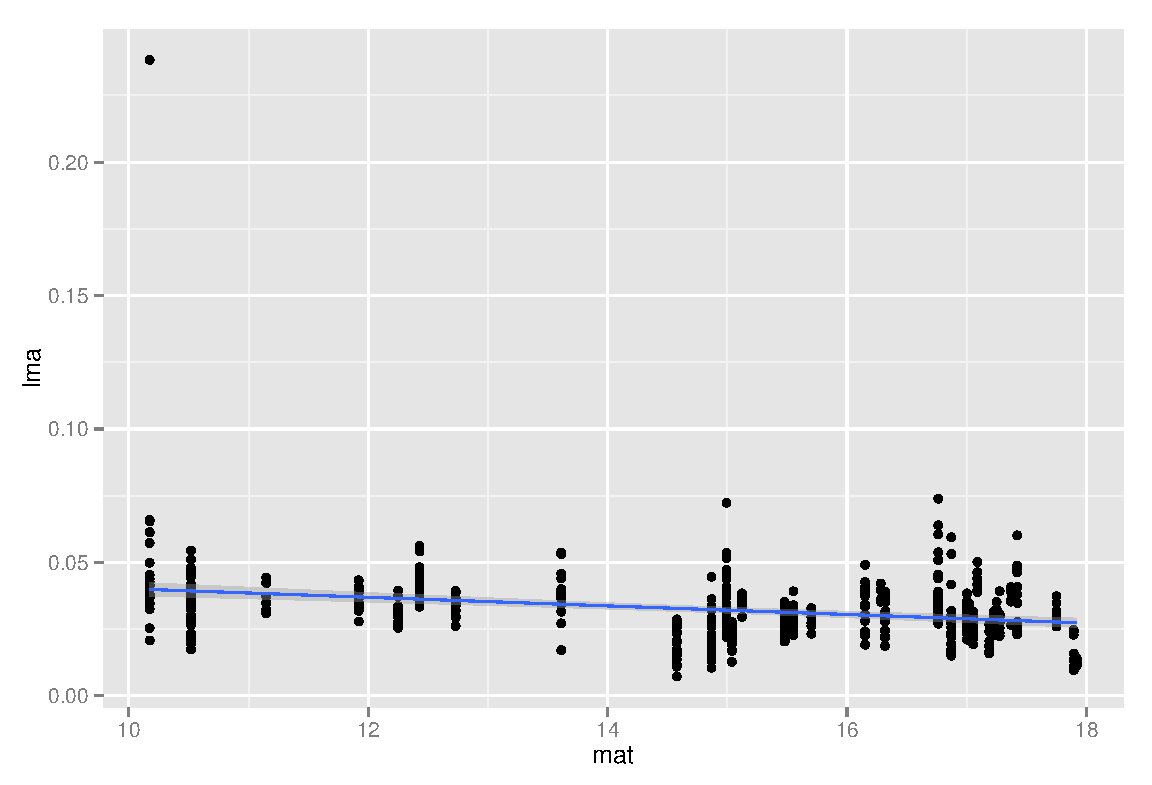
\includegraphics[height=5.5cm]{lma-outlier.pdf}
\end{center}

\item Could delete the observation if we have good evidence that it's
  an error.

\item Probably better to use an approach that leaves the data in and
  gives less weight to outliers.

\end{itemize}

\end{frame}

\begin{frame}{Robust Regression\footnote{robust-linear-regression.jags}}

\begin{itemize}

\item Use a Cauchy distribution (``fat tails'') instead of normal for
  prior on regression coefficients and residual error.\footnote{t
    distribution with 1 degree of freedom in JAGS}

\vfill

\begin{center}
\begin{tabular}{llcc}
\hline\hline
       &          &\multicolumn{2}{c}{Coefficient estimates} \\
Model  & Data set & $\beta_0$ & $\beta_{MAT}$ \\
\hline
Simple & Original & 0.000     & -0.313 \\
       & Modified & 0.028     & -0.372 \\
Robust & Original & -0.078    & -0.294 \\
       & Modified & -0.079    & -0.293 \\
\hline
\end{tabular}
\end{center}

\vfil

\item Estimates not affected by extreme outlier when using Cauchy
  prior.

\end{itemize}

\end{frame}

\begin{frame}{Multiple Linear Regression}

Simple generalization of what we've already seen
\begin{eqnarray*}
y_i &\sim& \mbox{N}(\mu_i, \sigma^2) \ ,  \\
\mu_i &=& \beta_0 + \sum_{k=1}^K\beta_kx_{ik} \ ,
\end{eqnarray*}
where $x_{ik}$ is the value of the $k$th covariate in individual
$i$. The priors are
\begin{eqnarray*}
\beta_k &\sim& \mbox{N}(0, \tau^{-1}), \quad k = 0,\dots,K \ , \\
\sigma^2 &=& \frac{1}{\tau_{resid}} \ ,  \\
\tau_{resid} &\sim& \mbox{Gamma}(1,\phi). 
\end{eqnarray*}

\end{frame}

\begin{frame}[fragile]{Multiple Linear Regression\footnote{multiple-linear-regression.jags}}

From JAGS
{\tiny
\begin{verbatim}
Inference for Bugs model at "multiple-linear-regression.jags", fit using jags,
 5 chains, each with 10000 iterations (first 5000 discarded), n.thin = 5
 n.sims = 5000 iterations saved
             mu.vect sd.vect     2.5%      25%      50%      75%    97.5%  Rhat n.eff
beta.0         0.000   0.040   -0.078   -0.027    0.000    0.028    0.078 1.001  4800
beta.cdd       0.106   0.073   -0.036    0.058    0.105    0.154    0.251 1.001  5000
beta.elev     -0.319   0.094   -0.500   -0.384   -0.319   -0.256   -0.136 1.001  5000
beta.inso      0.054   0.053   -0.048    0.018    0.054    0.091    0.157 1.001  5000
beta.map      -0.022   0.078   -0.178   -0.074   -0.020    0.031    0.129 1.001  5000
beta.mat      -0.463   0.114   -0.688   -0.541   -0.461   -0.385   -0.243 1.001  5000
beta.ratio    -0.016   0.079   -0.172   -0.069   -0.013    0.039    0.134 1.001  5000
sigma.resid    0.939   0.029    0.884    0.919    0.939    0.958    1.000 1.001  5000
\end{verbatim}
}

Compare to lm() from R
{\tiny
\begin{verbatim}
              Estimate Std. Error t value Pr(>|t|)
(Intercept) -3.520e-17  4.052e-02   0.000 1.000000
cdd          1.051e-01  7.315e-02   1.437 0.151291
elev        -3.184e-01  9.534e-02  -3.339 0.000899 ***
inso         5.288e-02  5.287e-02   1.000 0.317702
map         -2.309e-02  7.749e-02  -0.298 0.765836
mat         -4.629e-01  1.147e-01  -4.037  6.2e-05 ***
ratio       -1.481e-02  7.944e-02  -0.186 0.852218

Residual standard error: 0.9373 on 528 degrees of freedom
\end{verbatim}
}

\end{frame}

\begin{frame}{Multiple Linear Regression with Species Random Effect}

  $\gamma_i^{(s)}$ denotes the mean for species $s$ to which
  inidividual $i$ belongs
\begin{eqnarray*}
y_i &\sim& \mbox{N}(\mu_i, \sigma^2_{resid})\ ,  \\
\mu_i &=& \beta_0 + \sum_{k=1}^K\beta_kx_{ik} + \gamma_i^{(s)}\ , \\
\beta_k &\sim& \mbox{N}(0, \tau^{-1}), \quad k = 0,\dots,K \ , \\
\sigma^2_{resid} &=& \frac{1}{\tau_{resid}} \ ,  \\
\tau_{resid} &\sim& \mbox{Gamma}(1,\phi) \ , \\
\gamma_i^{(s)} &\sim& \mbox{N}(0, \sigma^2_{species}) \ ,  \\
\sigma^2_{species} &=& \frac{1}{\tau_{species}}\ ,  \\
\tau_{species} &\sim& \mbox{Gamma}(1,\phi) \ . 
\end{eqnarray*}

\end{frame}

\begin{frame}{Multiple Linear Regression with Species Random Effect}

Alternatively
\begin{eqnarray*}
y_i &\sim& \mbox{N}(\mu_i, \sigma^2_{resid})\ ,  \\
\mu_i &=& \beta_{0i}^{(s)} + \sum_{k=1}^K\beta_kx_{ik} \ , \\
\sigma^2_{resid} &=& \frac{1}{\tau_{resid}} \ , \\
\tau_{resid} &\sim& \mbox{Gamma}(1,\phi)\ ,  \\
\beta_{0i}^{(s)} &\sim& \mbox{N}(\beta_0, \sigma^2_{species}) \ ,  \\
\sigma^2_{species} &=& \frac{1}{\tau_{species}} \ , \\
\tau_{species} &\sim& \mbox{Gamma}(1,\phi) \ , \\
\beta_i &\sim& \mbox{N}(0, \tau), \quad i = 0,\dots,K\ . \\
\end{eqnarray*}

\end{frame}

\begin{frame}[fragile]{Multiple Linear Regression with Species Random
    Effect\footnote{random-effect-multiple-regression.jags}}

From JAGS
{\tiny
\begin{verbatim}
beta.cdd        0.081   0.055  -0.024   0.045   0.082   0.118   0.188 1.001  3100
beta.elev      -0.201   0.108  -0.408  -0.274  -0.201  -0.128   0.010 1.002  2400
beta.inso      -0.073   0.058  -0.187  -0.112  -0.073  -0.034   0.040 1.001  3400
beta.map       -0.418   0.083  -0.581  -0.474  -0.419  -0.362  -0.257 1.001  5000
beta.mat        0.093   0.110  -0.117   0.020   0.092   0.169   0.307 1.001  5000
beta.ratio      0.427   0.078   0.278   0.374   0.427   0.478   0.578 1.001  4800
beta.zero      -0.064   0.154  -0.369  -0.167  -0.062   0.037   0.241 1.001  5000
sigma.resid     0.545   0.023   0.511   0.532   0.544   0.556   0.581 1.001  3100
sigma.species   0.966   0.117   0.767   0.884   0.960   1.036   1.218 1.001  5000
\end{verbatim}
}
Compare to lmer() From R
{\tiny
\begin{verbatim}
Random effects:
 Groups   Name        Variance Std.Dev.
 species  (Intercept) 0.8951   0.9461
 Residual             0.2924   0.5408
Number of obs: 535, groups:  species, 42

Fixed effects:
            Estimate Std. Error t value
(Intercept) -0.06289    0.14898  -0.422
cdd          0.07941    0.05576   1.424
elev        -0.19835    0.10946  -1.812
inso        -0.07259    0.05791  -1.254
map         -0.42009    0.08176  -5.138
mat          0.09811    0.10893   0.901
ratio        0.43022    0.07776   5.533
\end{verbatim}
}

\end{frame}

\begin{frame}[fragile]{Multiple Linear Regression with Species Random
    Effect}

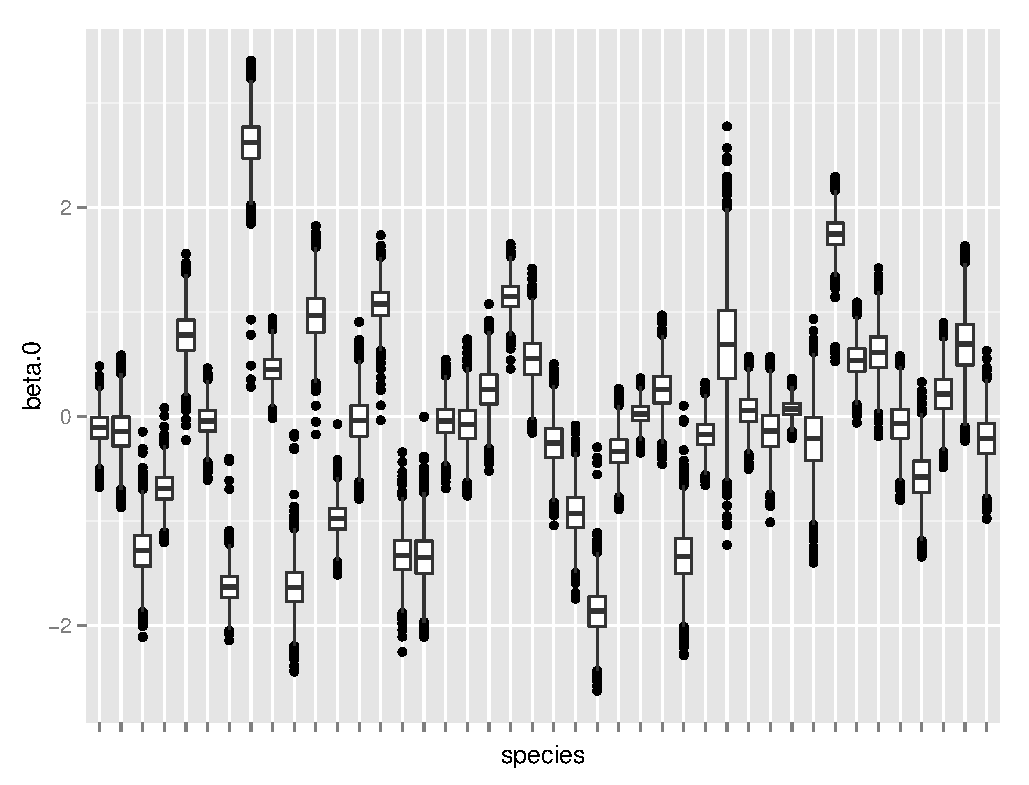
\includegraphics[height=8cm]{species-random-effect.pdf}

\end{frame}

\begin{frame}{Problems with Multicollinearity}
\begin{itemize}
\item Variables may appear to be unimportant (when they are).
\item  Coefficient estimates are unstable and hard to interpret (can estimate combinations of coefficients but not individual coefficients).
\end{itemize}

Alternative Bayesian solutions:
\begin{itemize}
\item Independent Prior Distributions
\item Variable Selection
\end{itemize}
\end{frame}

\begin{frame}{Hierarichal Model with Independent Priors}
Hierarchical Model:
\begin{equation*}
\begin{aligned}
\beta_j|\lambda_j,\sigma^2 &\sim \mbox{N}(0,\sigma^2/\lambda_j)\\
 \lambda_j|\sigma^2 &\sim \mbox{Gamma}(1/2,1/2)\\
1/\sigma^2 &\sim \mbox{Gamma}(\nu_0/2,\nu_0\sigma_0^2/2)
\end{aligned}
\end{equation*}

\begin{itemize}
% \item leads to nice conjugate updates for all full conditionals.
\item Leads to nice conjugate updates for all full conditionals
\item Easy to code in JAGS
\item Allows each parameter to have own precision with mean 1
\end{itemize}

\end{frame}

\begin{frame}{Cauchy Prior}
First two equations imply that $\beta_j |\sigma^2 \sim \mbox{Cauchy}(0,\sigma^2)$
\[
p(\beta)=\frac{1}{\pi\sigma}\left(1+\frac{\beta^2}{\sigma^2} \right)^{-1}, 
\]
leading to a collapsed model
\begin{equation*}
\begin{aligned}
Y|\boldsymbol\beta,\sigma^2 &\sim \mbox{N}({X\boldsymbol\beta},\sigma^2{I}_n)\ , \\
\beta_j|\sigma^2 &\sim \mbox{Cauchy}(0,\sigma^2)\ , \\
1/\sigma^2 &\sim \mbox{Gamma}(\nu_0/2,\nu_0\sigma_0^2/2) \ . 
\end{aligned}
\end{equation*}
No nice full conditional for $\beta_j$.
\end{frame}

\begin{frame}[fragile]{Cauchy Prior\footnote{hierarchical-prior-multiple-regression.jags}}

Independent $\mbox{N}(0, 1)$
{\tiny
\begin{verbatim}
beta.cdd        0.081   0.055  -0.024   0.045   0.082   0.118   0.188 1.001  3100
beta.elev      -0.201   0.108  -0.408  -0.274  -0.201  -0.128   0.010 1.002  2400
beta.inso      -0.073   0.058  -0.187  -0.112  -0.073  -0.034   0.040 1.001  3400
beta.map       -0.418   0.083  -0.581  -0.474  -0.419  -0.362  -0.257 1.001  5000
beta.mat        0.093   0.110  -0.117   0.020   0.092   0.169   0.307 1.001  5000
beta.ratio      0.427   0.078   0.278   0.374   0.427   0.478   0.578 1.001  4800
beta.zero      -0.064   0.154  -0.369  -0.167  -0.062   0.037   0.241 1.001  5000
sigma.resid     0.545   0.023   0.511   0.532   0.544   0.556   0.581 1.001  3100
sigma.species   0.966   0.117   0.767   0.884   0.960   1.036   1.218 1.001  5000
\end{verbatim}
}
Independent hierarchical
{\tiny
\begin{verbatim}
beta.cdd        0.084   0.055  -0.026   0.048   0.085   0.122   0.188 1.003  1300
beta.elev      -0.191   0.104  -0.394  -0.262  -0.190  -0.120   0.009 1.004   800
beta.inso      -0.077   0.059  -0.192  -0.117  -0.077  -0.038   0.039 1.001  5000
beta.map       -0.400   0.082  -0.562  -0.455  -0.401  -0.344  -0.240 1.004   870
beta.mat        0.084   0.107  -0.129   0.013   0.084   0.157   0.288 1.009   370
beta.ratio      0.416   0.079   0.262   0.363   0.417   0.469   0.570 1.007   510
beta.zero      -0.060   0.142  -0.338  -0.154  -0.061   0.035   0.224 1.002  2700
sigma.resid     0.545   0.018   0.512   0.533   0.544   0.556   0.580 1.001  5000
sigma.species   0.958   0.114   0.767   0.876   0.947   1.028   1.211 1.001  5000
\end{verbatim}
}

\end{frame}

\begin{frame}{Stochastic Search Variable Selection}
The Spike-and-Slab prior:
\begin{eqnarray*}
	\beta_j \mid \gamma_j, c, \tau_j^{-1} &\sim& (1-\gamma_j)\mathcal{N}(0, \tau_j^{-1})+\gamma_j \mathcal{N}(0, \tau_j^{-1} c^2) \ ,  \\
	\gamma_j \mid \pi_j &\sim& Bernoulli(\pi_j) \ . 
\end{eqnarray*}
\begin{columns}
\begin{column}{0.5\textwidth}
        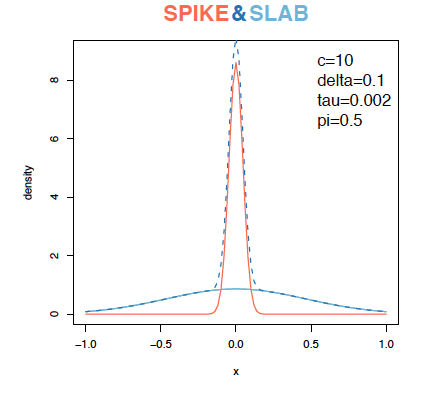
\includegraphics[scale=0.75]{SAS}
    \end{column}
    \begin{column}{0.47\textwidth}
        \begin{itemize}
            \item $\gamma_j=0$: Variable not in the model;
            \item $\gamma_j=1$:  Variable in the model;
            \item  Calibration of hyper-parameters $c$, $\tau_j^{-1}$ needed.
        \end{itemize}
    \end{column}
\end{columns}
\end{frame}

\begin{frame}
\begin{block}{Inference for Variable Selection}
\begin{itemize}
\item Highest posterior model (HPM): Select a model that has been visited most often.
\item Median probability model (MPM): Select variables that appear at least in 50\% of visited models.
\end{itemize}
\end{block}
\begin{block}{Alternative spike and slab models}
\begin{itemize}
\item Popular approach in genomic research;
\item Variants:
\begin{itemize}
\item Conjugate version:
\[
	\beta_j \mid \gamma_j, c, \tau_j^{-1} \sim (1-\gamma_j)\mathcal{N}(0, \sigma^2\tau_j^{-1})+\gamma_j \mathcal{N}(0, \sigma^2 \tau_j^{-1} c^2).
\]
\item Replace the spike normal in Spike-and-Slab prior by Dirac, i.e.,
\[
      \beta_j \mid \gamma_j, \tau_j^{-1} \sim (1-\gamma_j)\delta_0+\gamma_j \mathcal{N}(0, \tau_j^{-1}).
\]
\end{itemize}
\end{itemize}
\end{block}
\end{frame}

\begin{frame}[fragile]{Variable selection -- Dirac + Normal\footnote{dirac-plus-normal-multiple-regression.jags}}

Independent $\mbox{N}(0, 1)$
{\tiny
\begin{verbatim}
beta.cdd        0.081   0.055  -0.024   0.045   0.082   0.118   0.188 1.001  3100
beta.elev      -0.201   0.108  -0.408  -0.274  -0.201  -0.128   0.010 1.002  2400
beta.inso      -0.073   0.058  -0.187  -0.112  -0.073  -0.034   0.040 1.001  3400
beta.map       -0.418   0.083  -0.581  -0.474  -0.419  -0.362  -0.257 1.001  5000
beta.mat        0.093   0.110  -0.117   0.020   0.092   0.169   0.307 1.001  5000
beta.ratio      0.427   0.078   0.278   0.374   0.427   0.478   0.578 1.001  4800
beta.zero      -0.064   0.154  -0.369  -0.167  -0.062   0.037   0.241 1.001  5000
sigma.resid     0.545   0.023   0.511   0.532   0.544   0.556   0.581 1.001  3100
sigma.species   0.966   0.117   0.767   0.884   0.960   1.036   1.218 1.001  5000
\end{verbatim}
}
Dirac + $\mbox{N}(0,1)$
{\tiny
\begin{verbatim}
beta.cdd        0.002   0.015   0.000   0.000   0.000   0.000   0.039 1.029  1100
beta.elev      -0.277   0.112  -0.457  -0.349  -0.292  -0.224   0.000 1.016   310
beta.inso      -0.003   0.019  -0.052   0.000   0.000   0.000   0.000 1.054   460
beta.map       -0.473   0.075  -0.609  -0.523  -0.478  -0.429  -0.306 1.012   440
beta.mat        0.015   0.060   0.000   0.000   0.000   0.000   0.240 1.009  1100
beta.ratio      0.378   0.057   0.282   0.343   0.374   0.407   0.516 1.002  1800
beta.zero      -0.061   0.151  -0.355  -0.160  -0.060   0.039   0.240 1.001  5000
sigma.resid     0.546   0.023   0.512   0.533   0.545   0.557   0.581 1.001  5000
sigma.species   0.948   0.116   0.750   0.868   0.939   1.019   1.193 1.002  2100
\end{verbatim}
}

\end{frame}

\begin{frame}[fragile]{Variable selection -- Dirac + Normal}

Dirac + $\mbox{N}(0,1)$
{\tiny
\begin{verbatim}
beta.cdd        0.002   0.015   0.000   0.000   0.000   0.000   0.039 1.029  1100
beta.elev      -0.277   0.112  -0.457  -0.349  -0.292  -0.224   0.000 1.016   310
beta.inso      -0.003   0.019  -0.052   0.000   0.000   0.000   0.000 1.054   460
beta.map       -0.473   0.075  -0.609  -0.523  -0.478  -0.429  -0.306 1.012   440
beta.mat        0.015   0.060   0.000   0.000   0.000   0.000   0.240 1.009  1100
beta.ratio      0.378   0.057   0.282   0.343   0.374   0.407   0.516 1.002  1800
beta.zero      -0.061   0.151  -0.355  -0.160  -0.060   0.039   0.240 1.001  5000
sigma.resid     0.546   0.023   0.512   0.533   0.545   0.557   0.581 1.001  5000
sigma.species   0.948   0.116   0.750   0.868   0.939   1.019   1.193 1.002  2100
\end{verbatim}
}
Posterior conditioned on $\gamma_i > 0$
{\tiny
\begin{verbatim}
  beta.cdd:  0.04      0.057 (-0.042,  0.168)
 beta.elev:  0.93     -0.298 (-0.459, -0.134)*
 beta.inso:  0.05     -0.061 (-0.188,  0.059)
  beta.map:  1.00     -0.473 (-0.609, -0.306)*
  beta.mat:  0.11      0.142 (-0.111,  0.367)
beta.ratio:  1.00      0.379 ( 0.283,  0.516)*
\end{verbatim}
}
\end{frame}


\begin{frame}{Model Selection}
Selection of a single model has the following problems
\begin{itemize}
\item When the criteria suggest that several models are equally
good, what should we report? Still pick only one model?
\item What do we report for our uncertainty after selecting a model?
\end{itemize}
Typical analysis ignores model uncertainty!
\end{frame}

\begin{frame}{Bayesian Model Choice}
\begin{itemize}
\item Models for the variable selection problem are based on a
subset of the ${x}_1, \cdots, {x}_p$ variables.
\item Encode models with a vector $\boldsymbol\gamma=(\gamma_1, \cdots, \gamma_p)'$ where $\gamma_j \in \{0,1\}$ is an indicator for whether variable ${x}_j$ should be
included in the model $M_{\boldsymbol\gamma}$.  Notice $\gamma_j=0\Leftrightarrow \beta_j=0$.
\item Each value of $\boldsymbol\gamma$ represents one of the $2^p$ models.
\item Under model $M_{\boldsymbol\gamma}$:
\[
	{Y} \mid \boldsymbol\beta, \boldsymbol\gamma, \tau \sim \mathcal{N}({X}_{\boldsymbol\gamma}\boldsymbol\beta_{\boldsymbol\gamma}, \tau^{-1}{\bf I})
\]
where ${X}_{\boldsymbol\gamma}$ is the design matrix using the columns in $X$ where $\gamma_j=1$ and $\boldsymbol\beta_{\boldsymbol\gamma}$ is the subset of $\boldsymbol\beta$ that are non-zero.
\end{itemize}
\end{frame}

\begin{frame}{Bayesian Model Averaging}
Rather than use a single model, BMA uses all (or potentially a lot)
models, but weights model predictions by their posterior
probabilities (measure of how much each model is supported by
the data).
\begin{itemize}
\item Posterior model probabilities
\[
	{\rm P}(M_j \mid {Y})=\frac{{\rm P}({Y}\mid M_j){\rm P}(M_j)}{\sum_{j}{\rm P}({Y}\mid M_j){\rm P}(M_j)},
\]
Marginal likelihod of a model is
\[
	{\rm P}({Y}\mid M_{\boldsymbol\gamma})=\int \int {\rm P}({Y} \mid \boldsymbol\beta_{\boldsymbol\gamma}, \tau) {\rm P}(\boldsymbol\beta_{\boldsymbol\gamma} \mid \boldsymbol\gamma, \tau) {\rm P}(\tau \mid \boldsymbol\gamma) d\boldsymbol\beta_{\boldsymbol\gamma} d\tau.
\]
\item Probability $\beta_j\neq 0$: $\sum_{M_j: \beta_j\neq 0} {\rm P}(M_j \mid {Y})$.
\end{itemize}
\end{frame}

\begin{frame}{Bayesian Model Averaging (Continued)}
\begin{itemize}
\item Predictions
\[
	{\rm P}({Y}^{new} \mid {Y})=\sum_{j} {\rm P}({Y}^{new} \mid {Y}, M_j) {\rm P}(M_j \mid {Y}),
\]
where
\[
	{\rm P}({Y}^{new} \mid {Y}, M_{\boldsymbol\gamma})=\int {\rm P}({Y}^{new} \mid {Y}, \boldsymbol\beta_{\boldsymbol\gamma}, \tau) {\rm P}(\boldsymbol\beta_{\boldsymbol\gamma}, \tau \mid {Y}) d \boldsymbol\beta_{\boldsymbol\gamma} d\tau.
\]

\end{itemize}
\end{frame}

% \begin{frame}{Prior Distributions}
% \begin{itemize}
% \item Bayesian Model choice requires proper prior distributions on
% regression coefficients.
% \item Vague but proper priors may lead to paradoxes!
% % \item Conjugate Normal-Gammas lead to closed form expressions
% % for marginal likelihoods, Zellner's g-prior is the most popular.
% \end{itemize}
% \end{frame}

% \begin{frame}{Zellner's g-prior}
% Centered model:
% \[
% 		{\bf y}={\bf 1}_n \alpha+ \tilde{\bf X}_c\boldsymbol\beta+\boldsymbol\epsilon,
% \]
% where $\tilde{\bf X}_c=({\bf I}_n-1/n {\bf J}_n){\bf X}$ is the centered design matrix where all variables have had their mean subtracted.
% \begin{itemize}
% \item $\pi(\alpha)\propto 1$;
% \item $\pi(\tau)\propto 1/\tau$;
% \item $\boldsymbol\beta \mid \tau, \boldsymbol\gamma \sim \mathcal{N}({\bf 0}, g\tau^{-1} (\tilde{\bf X}_c'\tilde{\bf X}_c)^{-1})$;
% \item take $g=n$.
% \end{itemize}
% which leads to marginal likelihood of $M_{\boldsymbol\gamma}$ that is proportional to
% \[
% 	{\rm P}({\bf y} \mid M_{\boldsymbol\gamma}, g)\propto \frac{(1+g)^{(n-p_{\boldsymbol\gamma}-1)/2}}{(1+g(1-R_{\boldsymbol\gamma}^2))^{(n-1)/2}},
% \]
% where $R_{\boldsymbol\gamma}^2$ is the ordinary coefficient of determination of regression model $M_{\boldsymbol\gamma}$.

% Lastly, assign uniform distribution to space of models.
% \end{frame}



% \begin{frame}{Air Pollution Data}
% \begin{itemize}
% \item Response $SO_2$ measurements in $41$ metropolitan areas.
% \item Predictors:
% \begin{itemize}
% \item temp
% \item mfgfirms
% \item popn
% \item wind
% \item precip
% \item raindays
% \end{itemize}
% Model for $SO_2$ as a function of the other variables?
% \end{itemize}
% \end{frame}

% \begin{frame}{Scatterplot Matrix}
% Original Variables\\
% \begin{center}
% 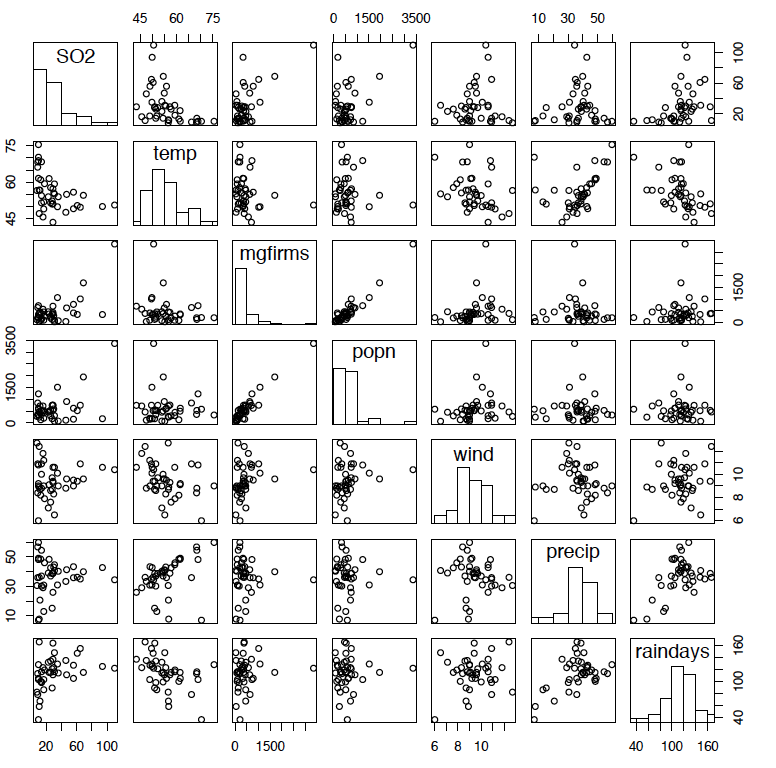
\includegraphics[scale=0.5]{SMP}
% \end{center}
% \end{frame}

% \begin{frame}{Scatterplot Matrix}
% Transformed Predictor Variables\\
% \begin{center}
% 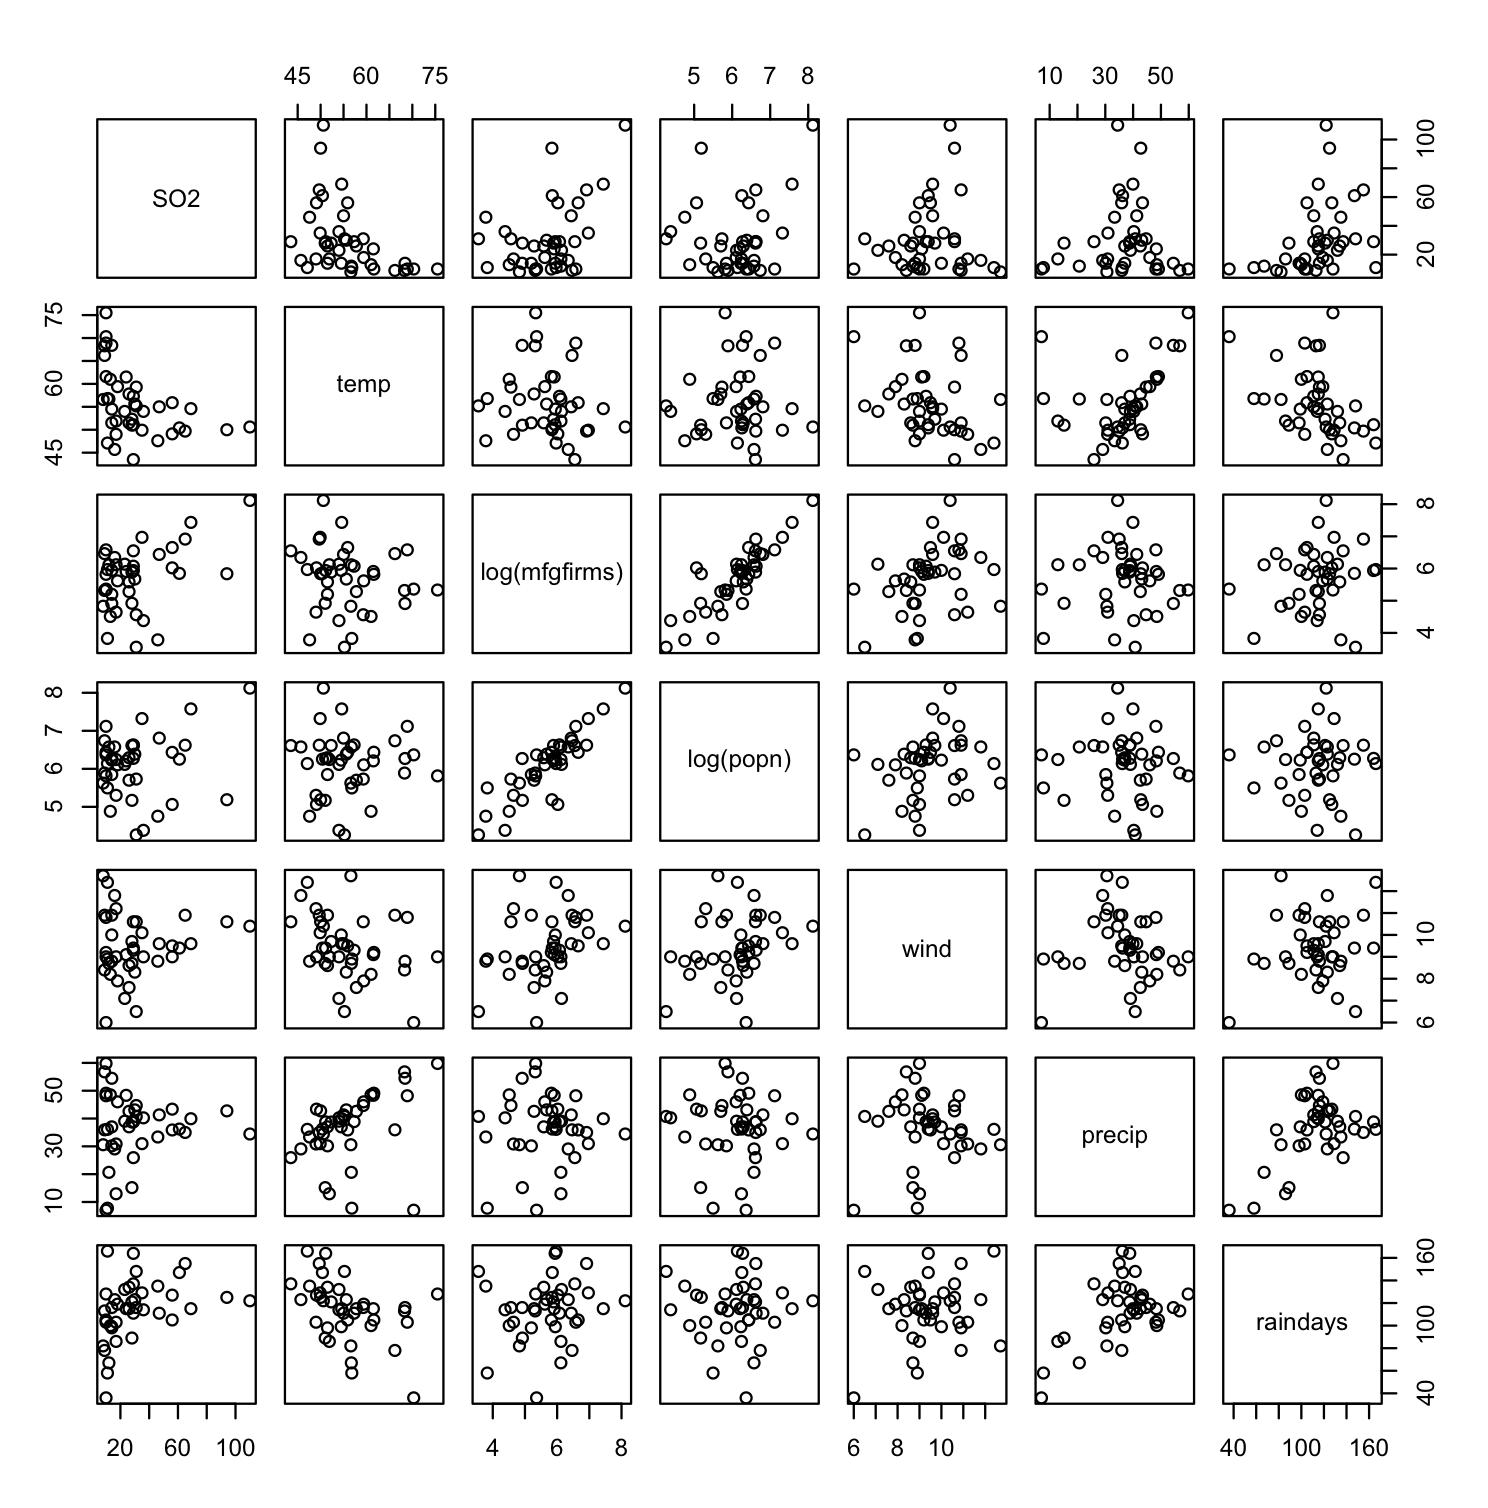
\includegraphics[scale=0.275]{p_22}
% \end{center}
% \end{frame}

% \begin{frame}{Residual Plots}
% \begin{center}
% 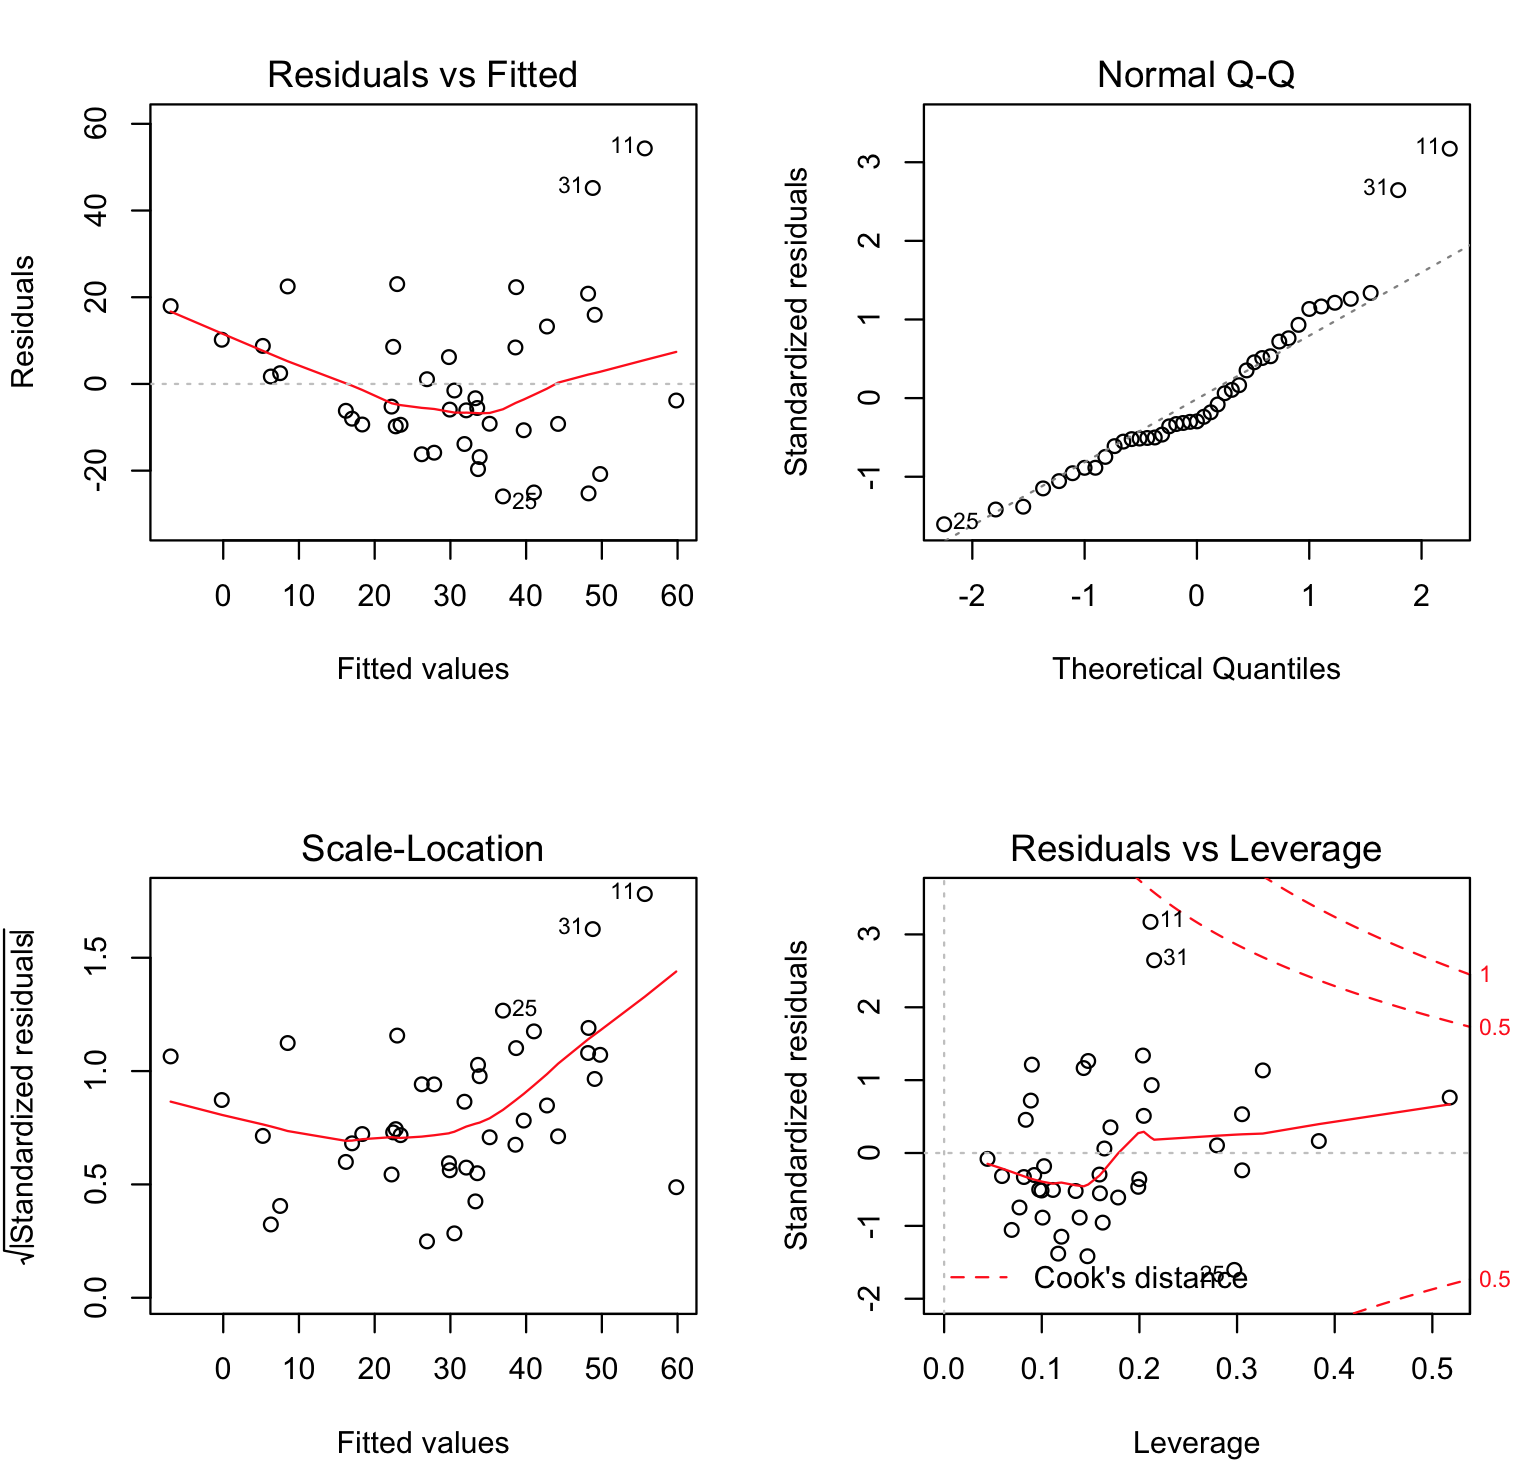
\includegraphics[scale=0.275]{p_21}
% \end{center}
% \end{frame}

% \begin{frame}{BoxCox Profile Likelihood}
% \begin{center}
% 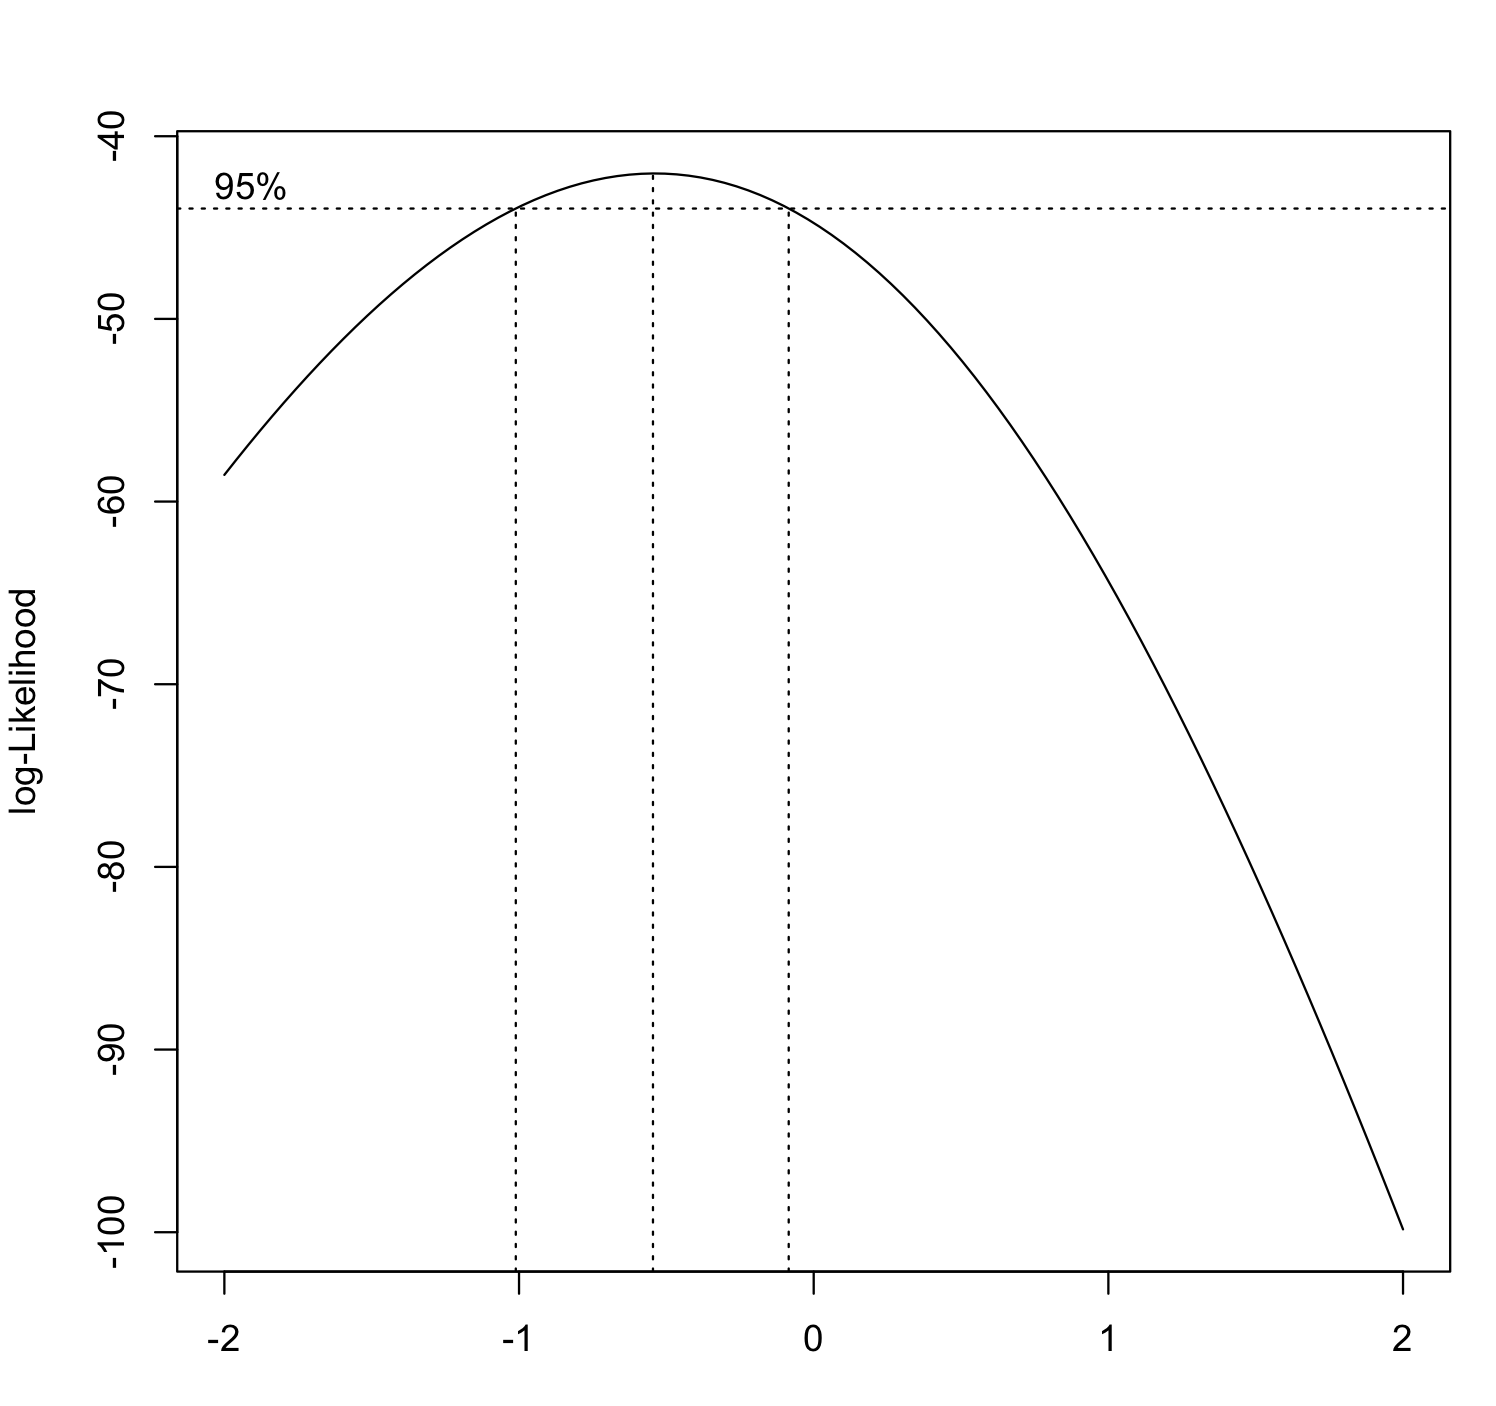
\includegraphics[scale=0.275]{p_bc}
% \end{center}
% $\lambda\approx-0.5$.
% \end{frame}

% \begin{frame}{Residual Plots}
% \begin{center}
% 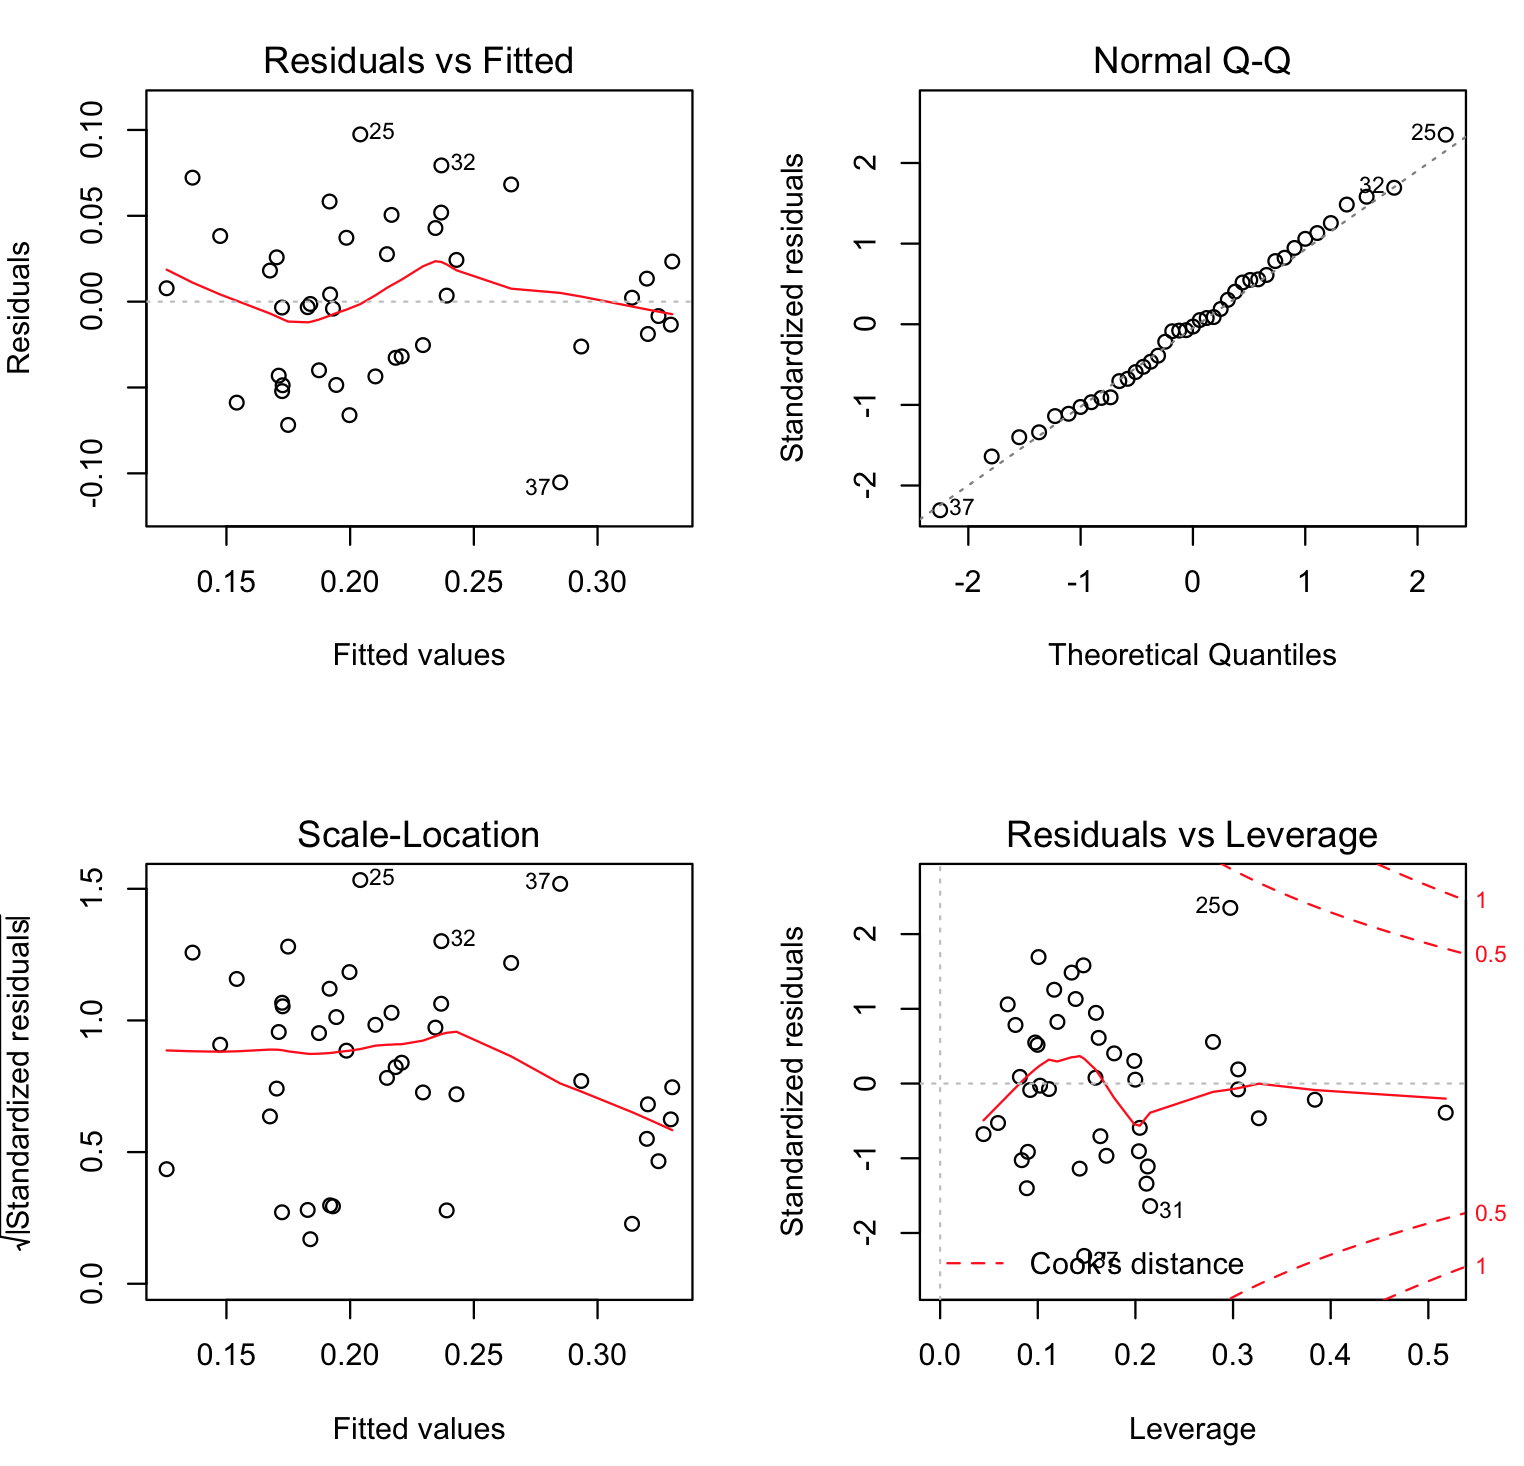
\includegraphics[scale=0.275]{p_23}
% \end{center}
% \end{frame}

% \begin{frame}
% \begin{table}[ht]
% \centering
% \caption{Least Squares Estimates of the Coefficients}
% \begin{tabular}{rrrrr}
%   \hline
%  & Estimate & Std. Error & t value & Pr($>$$|$t$|$) \\
%   \hline
% (Intercept) & -0.2287 & 0.1594 & -1.43 & 0.1605 \\
%   temp & 0.0076 & 0.0022 & 3.46 & {\color{red}0.0015} \\
%   log(mfgfirms) & -0.0284 & 0.0187 & -1.52 & 0.1389 \\
%   log(popn) & 0.0097 & 0.0226 & 0.43 & 0.6713 \\
%   wind & 0.0216 & 0.0064 & 3.39 & {\color{red}0.0018} \\
%   precip & -0.0018 & 0.0013 & -1.39 & 0.1746 \\
%   raindays & -0.0001 & 0.0006 & -0.21 & 0.8327 \\
%    \hline
% \end{tabular}
% \end{table}
% \end{frame}

% \begin{frame}{Pollution Example}
% \begin{itemize}
% \item Temperature is a significant predictor of $SO_2$ according to the $p$-value.
% \item Lower bound on Bayes Factor
% \[
% 	BF[H_0: H_a]=-e p \log(p)=0.027
% \]
% Here $p$ is the $p$-value.
% \item Strong evidence against that the ccoefficient of Temperature is zero.
% \end{itemize}
% \end{frame}

% \begin{frame}{USair Data}
% \begin{center}
% 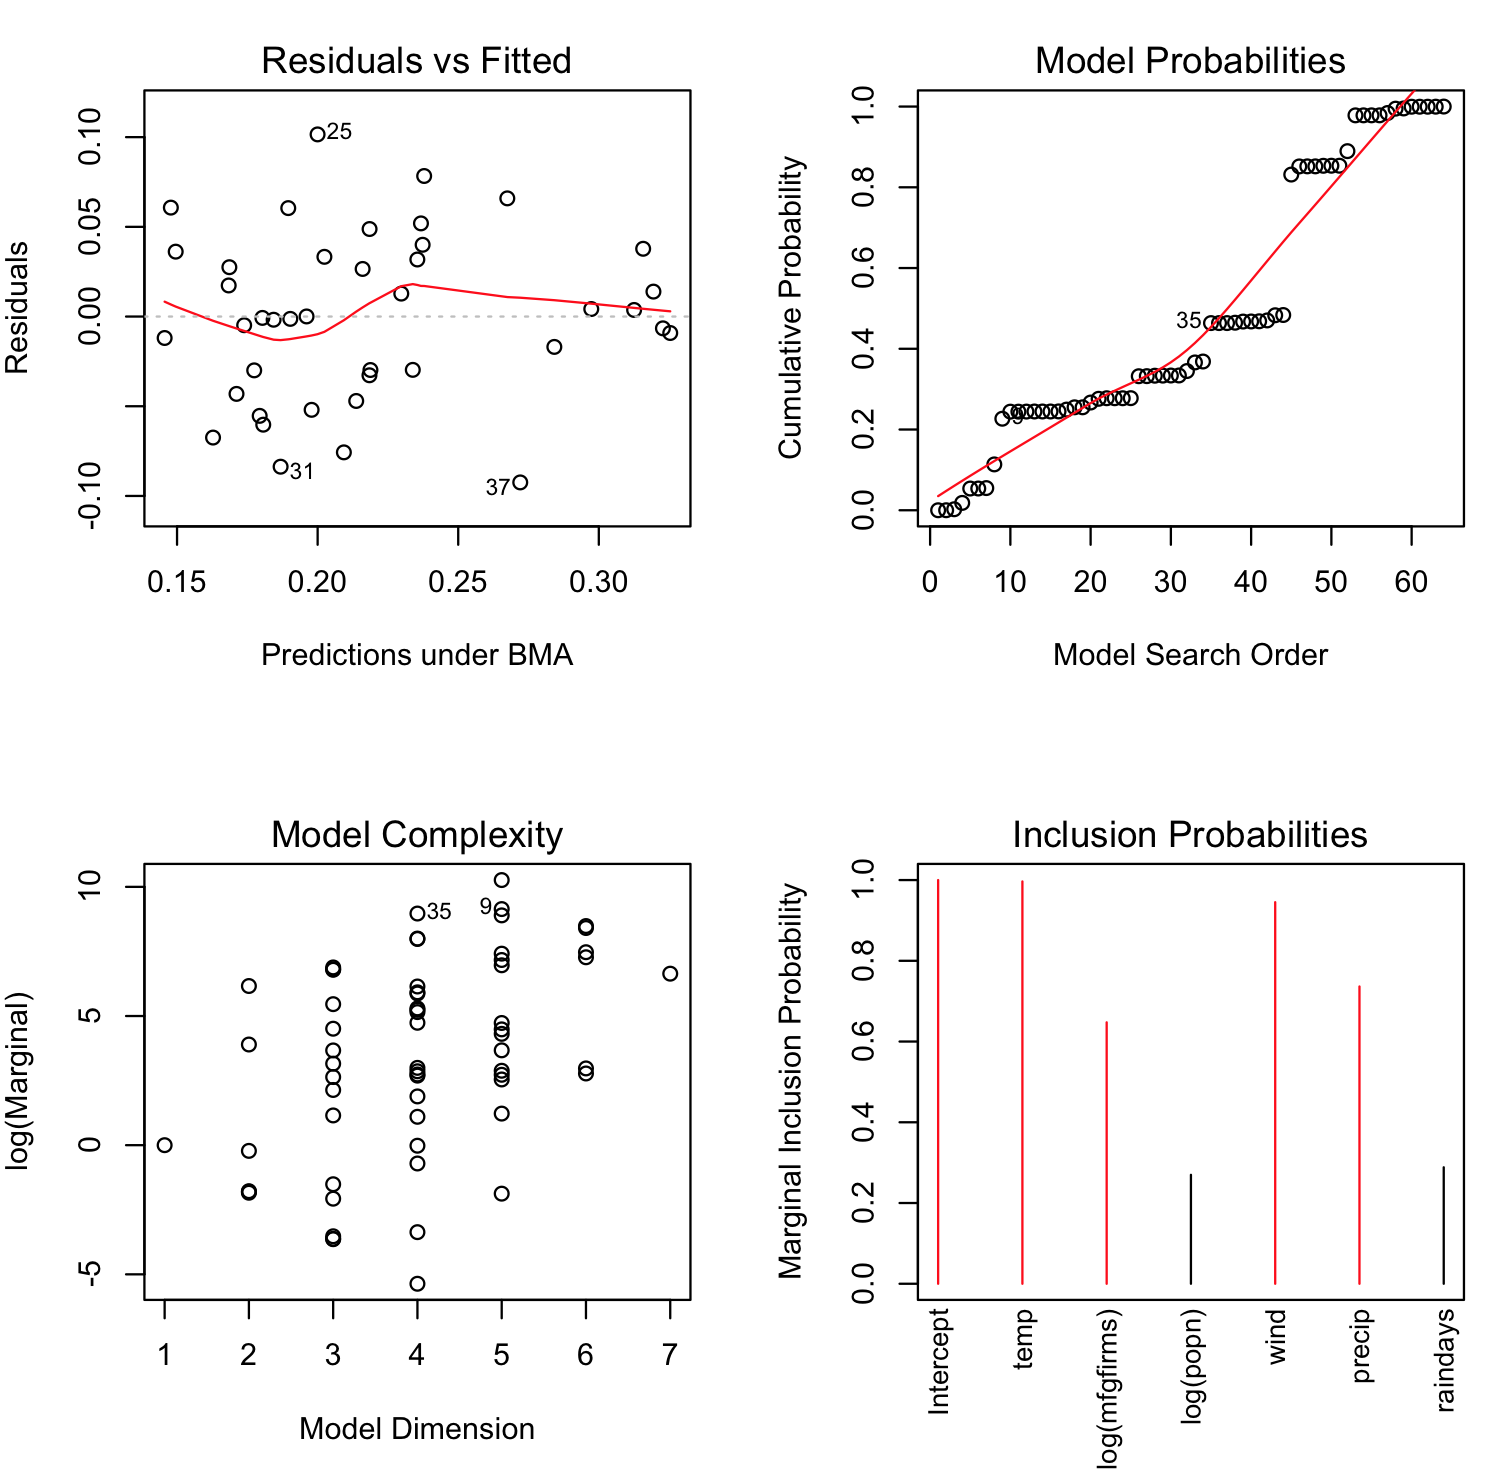
\includegraphics[scale=0.25]{p_a}
% \end{center}
% \end{frame}

% \begin{frame}{Model Space}
% \begin{center}
% 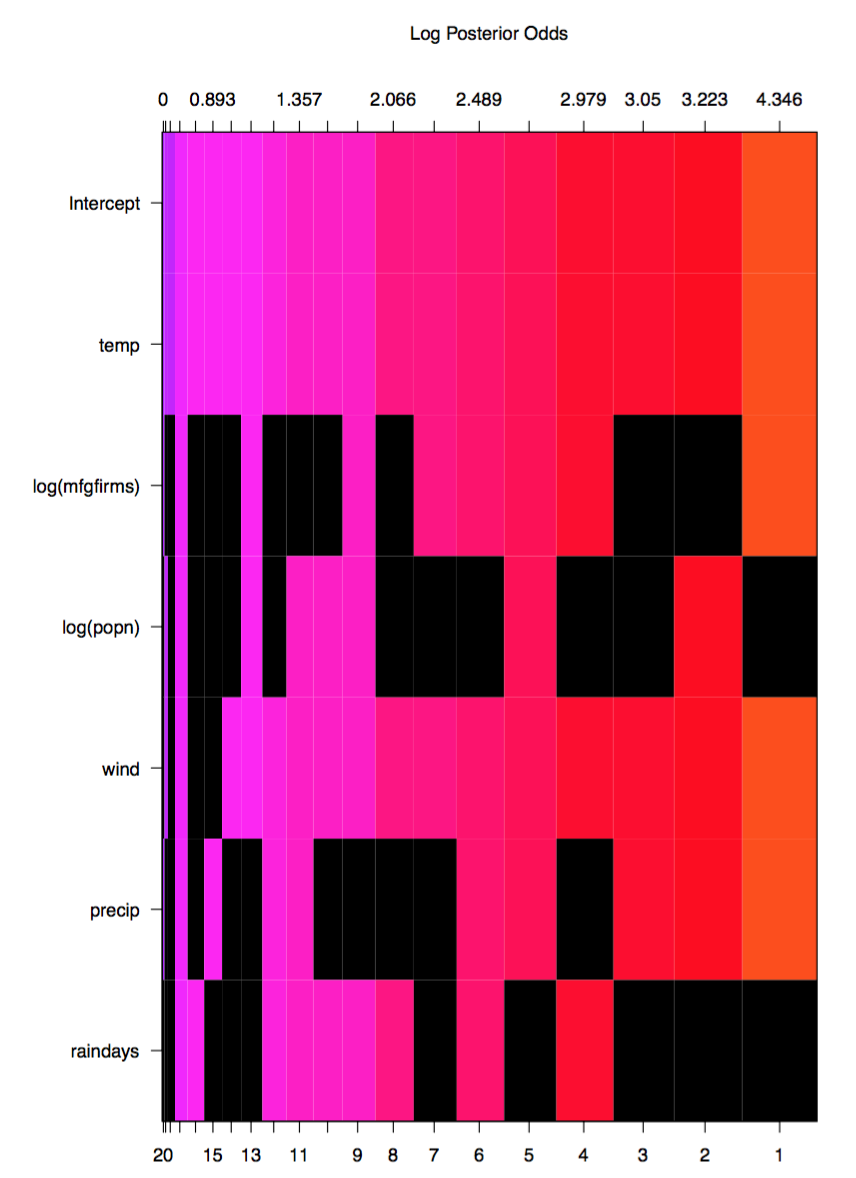
\includegraphics[scale=0.4]{poll_image}
% \end{center}
% \end{frame}

% \begin{frame}{Coefficient}
% \begin{center}
% 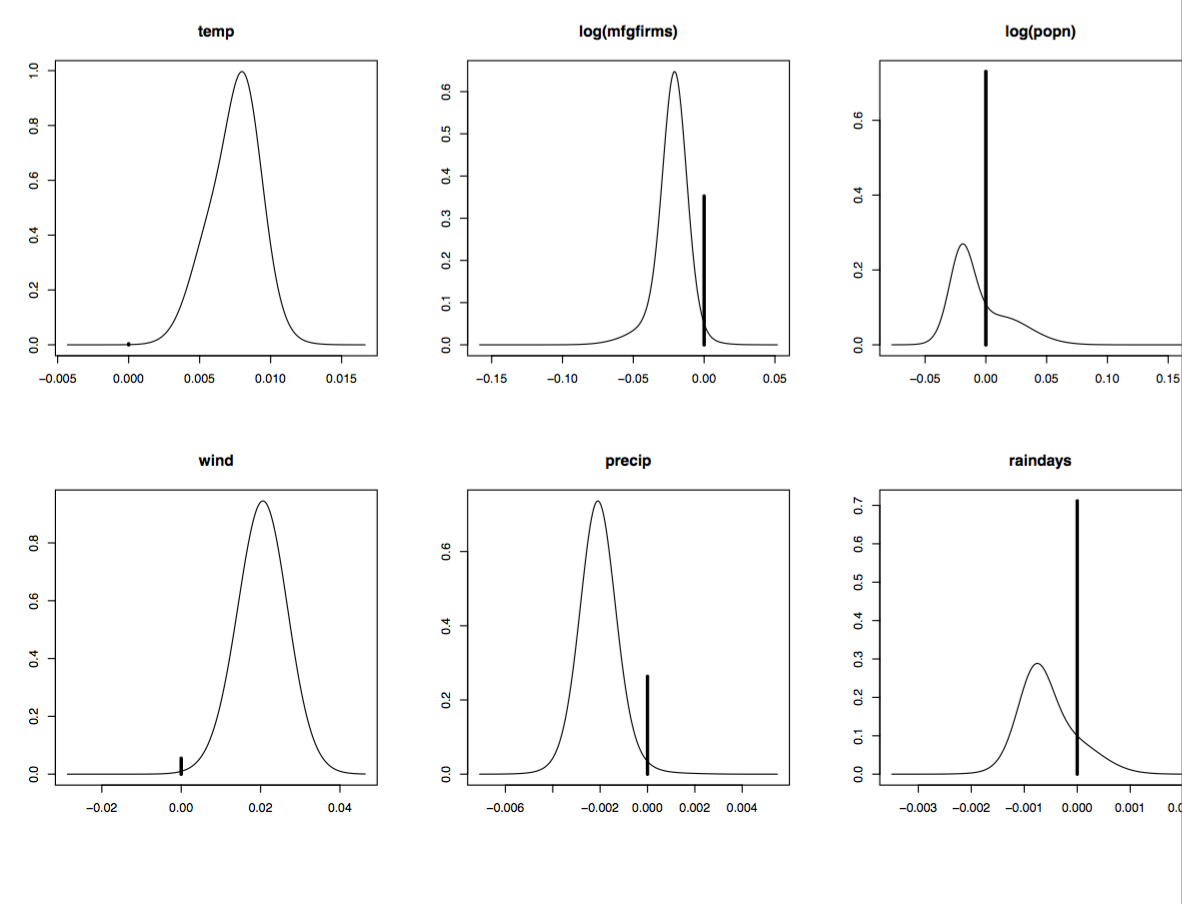
\includegraphics[scale=0.5]{poll_beta}
% \end{center}
% \end{frame}





\end{document}
